%%
%% (
%%  )\ )                             (
%%  (()/(   (            (             )\  )   (
%%   /(_))  ))\   (       ))\  (   (   (()/(   ))\
%%   (_))  /((_)  )\  )  /((_) )\  )\   ((_))/((_)
%%   | _ \(_))(  _(_/( (_) )  ((_)((_)  _| |(_))
%%   |   /| || || ' \))/ -_)/ _|/ _ \/ _` |/ -_)
%%   |_|_\ \_,_||_||_| \___|\__|\___/\__,_|\___|
%%

\documentclass{article}
\usepackage{fontspec}
\usepackage[utf8]{inputenc}
\usepackage{amsmath}
%\usepackage{slashbox}
\usepackage{amsfonts}
\usepackage{amssymb}
\usepackage{graphicx} % Paquete para incluir imágenes en el documento LaTeX
\usepackage{hyperref}
\hypersetup{
  colorlinks=true,
  linkcolor=blue,
  filecolor=magenta,
  urlcolor=cyan,
}
\urlstyle{same}
\usepackage{varwidth}

\newcommand\tab[1][1cm]{\hspace*{#1}}

\usepackage{multirow}

\usepackage[a4paper,rmargin=1.5cm,lmargin=1.5cm,top=1.5cm,bottom=1.5cm]{geometry}

\usepackage{pdfpages}

\usepackage{xcolor}
\usepackage{minted}
\setminted[css]{frame=lines, framesep=2mm, baselinestretch=1.2, rulecolor=\color{black!80},
                bgcolor=DarkGray,fontsize=\normalsize}
\usemintedstyle[css]{monokai}
\setminted[python]{frame=lines, framesep=2mm, baselinestretch=1.2, rulecolor=\color{black!80}, bgcolor=DarkGray}
\usemintedstyle[python]{monokai}
\setminted[java]{frame=lines, framesep=2mm, baselinestretch=1.2, rulecolor=\color{black!80}, bgcolor=DarkGray}
\usemintedstyle[java]{monokai}
\setminted[javascript]{frame=lines, framesep=2mm, baselinestretch=1.2, rulecolor=\color{black!80}, bgcolor=DarkGray}
\usemintedstyle[javascript]{monokai}
\setminted[php]{frame=lines, framesep=2mm, baselinestretch=1.2, rulecolor=\color{black!30}, bgcolor=LightGray}
\setminted[html]{frame=lines, framesep=2mm, baselinestretch=1.2, rulecolor=\color{black!30}, bgcolor=LightGray}
\setminted[bash]{baselinestretch=1.2,rulecolor=\color{black!30},bgcolor=LightGray}
\definecolor{LightGray}{gray}{0.98}
\definecolor{DarkGray}{gray}{0.1}
\definecolor{MidGray}{gray}{0.8}
\definecolor{codegreen}{rgb}{0,0.6,0}
\definecolor{codegray}{rgb}{0.5,0.5,0.5}
\definecolor{codepurple}{rgb}{0.58,0,0.82}
\definecolor{backcolour}{rgb}{0.95,0.95,0.92}
\setminted[json]{frame=lines, framesep=2mm, baselinestretch=1.2, rulecolor=\color{black!80}, bgcolor=DarkGray}
\usemintedstyle[json]{monokai}
\setminted[apacheconf]{frame=lines, framesep=2mm, baselinestretch=1.2, rulecolor=\color{black!30}, bgcolor=LightGray}
\setminted[html+twig]{frame=lines, framesep=2mm, baselinestretch=1.2, rulecolor=\color{black!30}, bgcolor=LightGray}
\setminted[html+php]{frame=lines, framesep=2mm, baselinestretch=1.2, rulecolor=\color{black!30}, bgcolor=LightGray}

%\setlength{\parindent}{0px}  % Setea la indentacion de la primera linea de cada parrafo a cero pixeles.


\title{Programación en Laravel}
\author{@RuneCode}

\begin{document}

%% Clase 1
\section{Intro y características}%
Laravel es un framework completo que cuenta con muchos módulos que te ayudarán
para el desarrollo de tus aplicaciones. Existen otros frameworks de PHP como
Symfony o Zend, sin embargo Laravel es uno de los líderes en el mercado.\\

Laravel no solo es sencillo y tiene muchas herramientas de desarrollo, sino que
también cuenta con una amplia comunidad a su alrededor; esta comunidad ha
logrado que sea posible tener una excelente documentación que puede ser
encontrada en Laracast y se ha creado un gran ecosistema con foros y
comunidades.\\
También existen proyectos que se han desarrollado a partir de Laravel como
Lumen que es un micro-framework o Spark que te da un punto de inicio para
aplicaciones de cobros.\\

En este curso se trabajará pensando que ya tienes bases de PHP. Si no tienes
estas bases, puedes adquirirlas en el curso de Platzi de Introducción a PHP.\\
El proyecto del curso será crear un sistema para reporte de gastos.\\

%% Clase 2
\section{Instalación de Laravel}%
Composer es un manejador de dependencias para PHP, así que todas las
dependencias que necesitemos, incluído Laravel, serán instaladas por
Composer.
Para trabajar en Laravel necesitarás un servidor de PHP y una base de datos.\\
Laravel nos ofrece un instalador que podemos traer a través de Composer y
utilizaremos global en el comando para que la instalación se realice en toda la
máquina virtual o computador.
Podemos comprobar si Laravel quedó bien instalado usando el comando "laravel"
el cual nos dará la versión del instalador y los comandos disponibles.
El comando "new" nos ayuda a crear un nuevo proyecto de Laravel; al hacer esto
se crearán las carpetas y estructura del proyecto y el archivo composer con las
dependencias necesarias.
Para trabajar con Laravel es necesario tener la versión de PHP 7.1 o
superior.
El comando "artisan" nos da una serie de comandos de Laravel, son muchos y no
todos se utilizan pero es buena idea revisar la documentación y opciones
disponibles.
El comando "serve" levanta un servidor de PHP corriendo el proyecto actual, el
cual nos arroja una dirección IP la cual abriéndola nos muestra nuestro
proyecto.\\


\begin{figure}[h!]
  \centering
  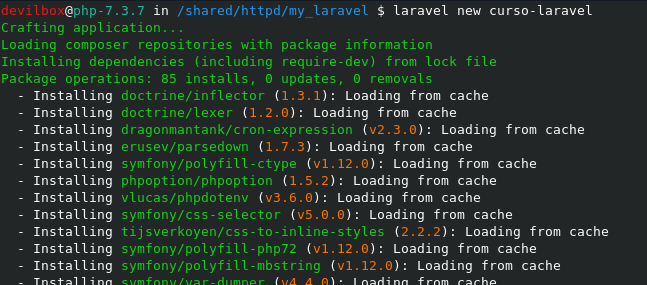
\includegraphics[scale=0.75]{./Pictures/001_Install_laravel.png}
\end{figure}

\begin{figure}[h!]
  \centering
  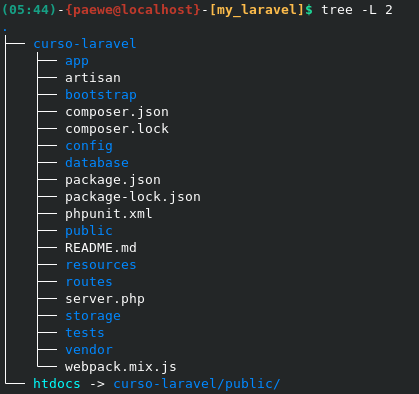
\includegraphics[scale=0.65]{./Pictures/002_estructura.png}
\end{figure}

\newpage

\begin{figure}[h!]
  \centering
  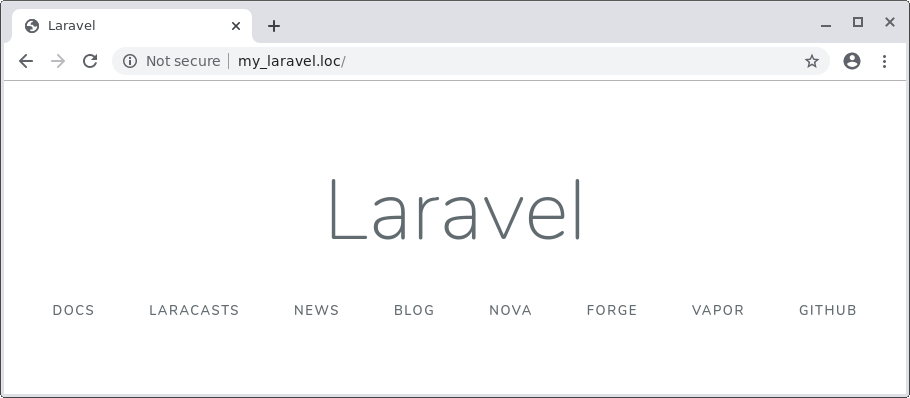
\includegraphics[scale=0.5]{./Pictures/003_laravel.png}
\end{figure}


%% Clase 3
\section{Primera ruta en Laravel}%
Laravel cuenta con un mecanismo para generar rutas y especificar el método que
queremos utilizar (get, post, put…) teniendo la posibilidad de incluso
mezclarlos.\\

\begin{itemize}
  \item En el archivo web.php encontramos todas las rutas que trabajaremos.
  \item Las vistas se encuentran dentro de resources/views.
  \item Las vistas básicas se realizan utilizando closures.
  \item Podemos regresar vistas, textos, arreglos asociativos, entre otros;
    devolviendo los arreglos en formato json lo cual es muy útil al momento de
    realizar pruebas.
  \item Es en web.php donde podemos definir el método que vamos a usar.
\end{itemize}


\textbf{routes/web.php}
\begin{minted}{php}
  <?php

  /*
  |--------------------------------------------------------------------------
  | Web Routes
  |--------------------------------------------------------------------------
  |
  | Here is where you can register web routes for your application. These
  | routes are loaded by the RouteServiceProvider within a group which
  | contains the "web" middleware group. Now create something great!
  |
  */

  Route::get('/', function () {
      return view('welcome');
  });

  Route::get('/test', function () {
    return "Hola Platzi";
  });
\end{minted}


\begin{figure}[h!]
  \centering
  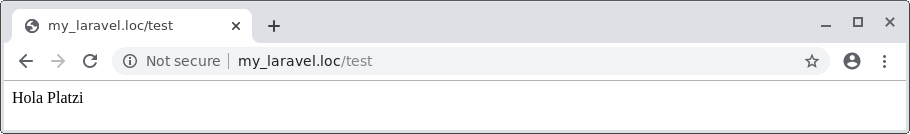
\includegraphics[scale=0.5]{./Pictures/004_test.png}
\end{figure}

\textbf{routes/web.php}
\begin{minted}{php}
  <?php

  /*
  |--------------------------------------------------------------------------
  | Web Routes
  |--------------------------------------------------------------------------
  |
  | Here is where you can register web routes for your application. These
  | routes are loaded by the RouteServiceProvider within a group which
  | contains the "web" middleware group. Now create something great!
  |
  */

  Route::get('/', function () {
      return view('welcome');
  });

  Route::get('/test', function () {
    return [
      'saludo' => 'Hola',
      'nombre' => 'Platzi'
    ];
  });
\end{minted}

\begin{figure}[h!]
  \centering
  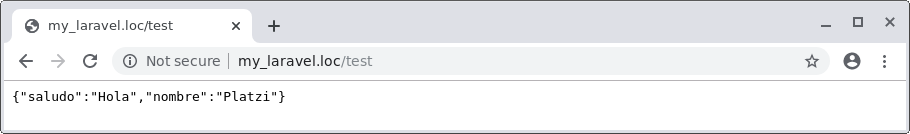
\includegraphics[scale=0.5]{./Pictures/005_laravel_json.png}
\end{figure}

\textbf{resources/views/welcome.blade.php}
\begin{minted}{html+php}
  <!DOCTYPE html>
  <html lang="{{ str_replace('_', '-', app()->getLocale()) }}">
      <head>
          <meta charset="utf-8">
          <meta name="viewport" content="width=device-width, initial-scale=1">

          <title>Laravel</title>

          <!-- Fonts -->
          <link href="https://fonts.googleapis.com/css?family=Nunito:200,600" rel="stylesheet">

          <!-- Styles -->
          <style>
              html, body {
                  background-color: #fff;
                  color: #636b6f;
                  font-family: 'Nunito', sans-serif;
                  font-weight: 200;
                  height: 100vh;
                  margin: 0;
              }

              .full-height {
                  height: 100vh;
              }

              .flex-center {
                  align-items: center;
                  display: flex;
                  justify-content: center;
              }

              .position-ref {
                  position: relative;
              }

              .top-right {
                  position: absolute;
                  right: 10px;
                  top: 18px;
              }

              .content {
                  text-align: center;
              }

              .title {
                  font-size: 84px;
              }

              .links > a {
                  color: #636b6f;
                  padding: 0 25px;
                  font-size: 13px;
                  font-weight: 600;
                  letter-spacing: .1rem;
                  text-decoration: none;
                  text-transform: uppercase;
              }

              .m-b-md {
                  margin-bottom: 30px;
              }
          </style>
      </head>
      <body>
          <div class="flex-center position-ref full-height">
              @if (Route::has('login'))
                  <div class="top-right links">
                      @auth
                          <a href="{{ url('/home') }}">Home</a>
                      @else
                          <a href="{{ route('login') }}">Login</a>

                          @if (Route::has('register'))
                              <a href="{{ route('register') }}">Register</a>
                          @endif
                      @endauth
                  </div>
              @endif

              <div class="content">
                  <div class="title m-b-md">
                      Curso Laravel
                  </div>

                  <div class="links">
                      <a href="https://laravel.com/docs">Docs</a>
                      <a href="https://laracasts.com">Laracasts</a>
                      <a href="https://laravel-news.com">News</a>
                      <a href="https://blog.laravel.com">Blog</a>
                      <a href="https://nova.laravel.com">Nova</a>
                      <a href="https://forge.laravel.com">Forge</a>
                      <a href="https://vapor.laravel.com">Vapor</a>
                      <a href="https://github.com/laravel/laravel">GitHub</a>
                  </div>
              </div>
          </div>
      </body>
  </html>
\end{minted}

\begin{figure}[h!]
  \centering
  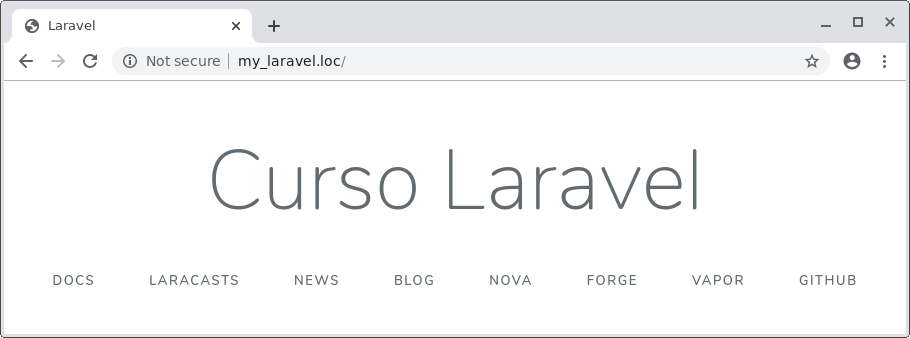
\includegraphics[scale=0.5]{./Pictures/006_vistas.png}
\end{figure}

\textbf{routes/web.php}
\begin{minted}{php}
  <?php

  /*
  |--------------------------------------------------------------------------
  | Web Routes
  |--------------------------------------------------------------------------
  |
  | Here is where you can register web routes for your application. These
  | routes are loaded by the RouteServiceProvider within a group which
  | contains the "web" middleware group. Now create something great!
  |
  */

  Route::get('/', function () {
      return view('welcome');
  });

  Route::get('/test', function () {
    return view('test');
  });
\end{minted}

\textbf{resources/views/test.blade.php}
\begin{minted}{php}
  <!DOCTYPE html>
  <html lang="{{ str_replace('_', '-', app()->getLocale()) }}">
      <head>
          <meta charset="utf-8">
          <meta name="viewport" content="width=device-width, initial-scale=1">

          <title>Laravel</title>

          <!-- Fonts -->
          <link href="https://fonts.googleapis.com/css?family=Nunito:200,600" rel="stylesheet">

          <!-- Styles -->
          <style>
              html, body {
                  background-color: #fff;
                  color: #636b6f;
                  font-family: 'Nunito', sans-serif;
                  font-weight: 200;
                  height: 100vh;
                  margin: 0;
              }

              .full-height {
                  height: 100vh;
              }

              .flex-center {
                  align-items: center;
                  display: flex;
                  justify-content: center;
              }

              .position-ref {
                  position: relative;
              }

              .top-right {
                  position: absolute;
                  right: 10px;
                  top: 18px;
              }

              .content {
                  text-align: center;
              }

              .title {
                  font-size: 84px;
              }

              .links > a {
                  color: #636b6f;
                  padding: 0 25px;
                  font-size: 13px;
                  font-weight: 600;
                  letter-spacing: .1rem;
                  text-decoration: none;
                  text-transform: uppercase;
              }

              .m-b-md {
                  margin-bottom: 30px;
              }
          </style>
      </head>
      <body>
          <div class="flex-center position-ref full-height">
              @if (Route::has('login'))
                  <div class="top-right links">
                      @auth
                          <a href="{{ url('/home') }}">Home</a>
                      @else
                          <a href="{{ route('login') }}">Login</a>

                          @if (Route::has('register'))
                              <a href="{{ route('register') }}">Register</a>
                          @endif
                      @endauth
                  </div>
              @endif

              <div class="content">
                  <div class="title m-b-md">
                      Curso Laravel en Platzi
                  </div>

                  <div class="links">
                      <a href="https://laravel.com/docs">Docs</a>
                      <a href="https://laracasts.com">Laracasts</a>
                      <a href="https://laravel-news.com">News</a>
                      <a href="https://blog.laravel.com">Blog</a>
                      <a href="https://nova.laravel.com">Nova</a>
                      <a href="https://forge.laravel.com">Forge</a>
                      <a href="https://vapor.laravel.com">Vapor</a>
                      <a href="https://github.com/laravel/laravel">GitHub</a>
                  </div>
              </div>
          </div>
      </body>
  </html>
\end{minted}

\begin{figure}[h!]
  \centering
  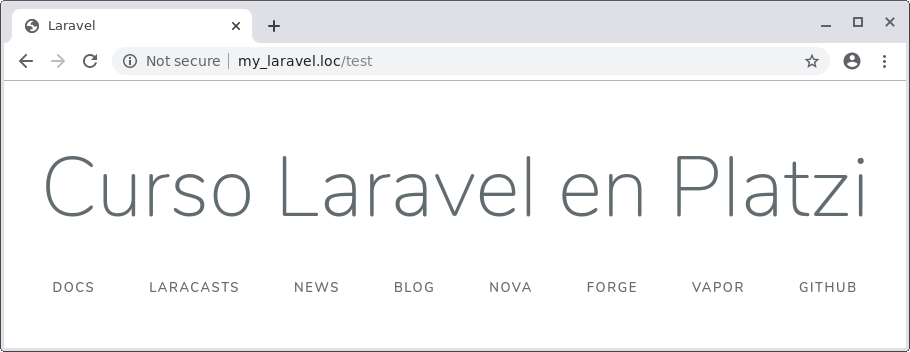
\includegraphics[scale=0.5]{./Pictures/007_test_vistas.png}
\end{figure}


%% Clase 4
\section{Cómo funciona Blade}%
Internamente Laravel utiliza un motor de render llamado Blade y utilizamos este
tipo motores porque PHP ha ido evolucionando más su parte de programación pero
no tanto su parte de motores de templates. Algunas librerías han sido creadas
para solventar esa falencia.\\

\begin{itemize}
  \item En nuestras vistas podremos encontrar estructuras de control como @if o
    @auth que son helpers de Blade.
  \item Cuando queremos enviar información desde nuestras rutas a nuestras
    vistas podemos hacerlo mediante arreglos asociativos en el archivo web.php,
    los cuales pueden ser mostrados como variables en las vistas.
  \item No es recomendado usar PHP dentro de Blade ya que para esto contamos
    con los helpers.
\end{itemize}




\end{document}

